\documentclass[11pt,a4paper]{article}  % Déclare la classe du document.

\newcommand{\chaptermark}[2]{\og #2 \fg{} (#1)} % ligne uniquement pour éviter une erreur en cas d'article
\usepackage[table,dvipsnames,svgnames]{xcolor}
\usepackage{listingsutf8}
%\usepackage[utf8]{inputenc}% gestion des accents (source)
\usepackage[T1]{fontenc}% gestion des accents (PDF)
\usepackage{fontspec}
\usepackage[french]{babel}% gestion du français
\usepackage{textcomp}% caractères additionnels
\usepackage{mathtools,amssymb,amsthm}% packages de l'AMS + mathtools
\usepackage{amsmath}
\usepackage{yhmath}
\usepackage{mathpazo}
\usepackage[scaled=0.95]{helvet}
\usepackage{courier}
%\usepackage{fourier}
%\usepackage[scaled=0.95]{helvet}
%\usepackage{courier}
\usepackage{bm}
\usepackage{gensymb}
\usepackage{graphicx}

\usepackage{enumitem}
\usepackage{pifont}

\usepackage{pstricks}
\usepackage{pstricks-add}
\usepackage{pst-eucl}
\usepackage{pgfplots}
\let\clipbox\relax
%\usepackage{pst-plot,pst-text,pst-tree,pstricks-add}
%\usepackage{pst-node} % required package
\usepackage{pst-all}
\usepackage[most,skins,breakable]{tcolorbox}

\usepackage{euscript}





% ############### Nouvelles commandes ###############
% Coloration des labels des points dans pst-eucl
\makeatletter
\define@key[psset]{pst-eucl}{LabelColor}{\def\psk@LabelColor{#1}}
\psset{LabelColor=black}
\def\Pst@WhichLabel#1{{\color{\psk@LabelColor}%
		\ifx\psk@PointName\@default#1\else\psk@PointName\fi}}
\makeatother

% renomme le symbole #2 en #1#2 et invalide le symbole initial #2:
\def\renamesymbol#1#2{
	\expandafter\let\expandafter\newsym\expandafter=\csname#2\endcsname
	\expandafter\global\expandafter\let\csname#1#2\endcsname=\newsym
	\expandafter\global\expandafter\let\csname#2\endcsname=\origsym
}



\usepackage{ProfCollege}
\renamesymbol{Casio}{Calculatrice}
\usepackage[nonshellescape]{ProfLycee}



%\usepackage[left=1.5cm,right=1.5cm,top=2.5cm,bottom=2.5cm]{geometry}
\usepackage[left=13mm,right=13mm,top=18mm,bottom=18mm,footskip=30pt]{geometry}
\setlength{\headheight}{15pt}

\usepackage{titlesec}
\usepackage{pas-math}
\usepackage{longtable}
\usepackage{tikz,tkz-tab}
\usepackage{amsmath}
\usepackage[right]{eurosym}
\usepackage{sectsty}
\usepackage{tipfr}
\usepackage{setspace}

%pour faire les touches de la calculatrices
\usepackage{menukeys}
\renewmenumacro{\menu}{roundedmenus} % default: menus
\renewmenumacro{\directory}{pathswithfolder} % default: paths
\renewmenumacro{\keys}{shadowedroundedkeys} % default: roundedkeys


\usepackage{multicol}
\usepackage{multirow}
\usepackage{systeme}

%% Format des titres de chapitres, paragraphes, ...
\titleformat{\chapter}[frame]
{\color{red!85!white}\normalsize}%
{\filright\sffamily\Large%
	\enspace Chapitre \thechapter\enspace}%
{8pt}
{\color{red!85!white}\rule{0pt}{30pt}\sffamily\Huge\bfseries\filcenter}
%%%%%%%%%%%%%%%%%%%%
\titlespacing{\chapter}{0pc}{0pc}{2pc}
\titlespacing{\subsection}{2pc}{}{}

\titleformat{\subsection}[block]{\hspace{1em}}{\thesubsection}{1em .}{}
\titleformat{\subsubsection}[block]{\hspace{2em}}{\thesubsection}{1em )}{}

\chapterfont{\color{red}{}}
\sectionfont{\color{green!55!black}{}}
\subsectionfont{\color{cyan!65!black}{}}
\subsubsectionfont{\color{violet}{}}
\renewcommand{\thesection}{\color{green!55!black}\Roman{section}.}
\renewcommand{\thesubsection}{\color{cyan!65!black}\arabic{subsection})}
\renewcommand{\thesubsubsection}{\color{violet}\alph{subsubsection})}
\setcounter{secnumdepth}{3}

\titleformat{\subsection}[block]{\hspace{1em}}{\thesubsection}{1em .}{}
\titleformat{\subsubsection}[block]{\hspace{2em}}{\thesubsection}{1em )}{}

\usepackage[column=A]{cellspace}
\setlength{\cellspacebottomlimit}{4pt}
\setlength{\cellspacetoplimit}{4pt}
\setlength{\parindent}{2pt}
\setlength{\tabcolsep}{0.5cm}


%entête et pieds de pages
\usepackage{fancyhdr}
\pagestyle{fancy}
\fancyhf{}
\usepackage{lastpage}
\renewcommand{\chaptermark}[1]{\markboth {Chapitre \thechapter~ - ~#1}{}}
\renewcommand\headrulewidth{1pt}
\fancyhead[LO,RE]{Terminale $-$ Maths complémentaire}
\fancyhead[RO,LE]{\leftmark}
\renewcommand\footrulewidth{1pt}
\fancyfoot[LO,RE]{Année 2025-2026}
\fancyfoot[RO,LE]{\textbf{Page \thepage/\pageref{LastPage}}}

%Mes boites pour les définitions, propriétés, remarques, ...

%Mes boites pour les définitions, propriétés, remarques, ...

\newcommand\titrebox[1]{\textbf{#1}}
\newtcolorbox{definition}{breakable,colback=red!10!white,
	colframe=red!85!white, fonttitle=\bfseries,enhanced,
	attach boxed title to top left={xshift=5mm, yshift=-2mm},boxed title style={size=small,colback=red!10!white,colframe=red!85!white, arc=0.5mm},
	title=\textcolor{red!85!white}{Définition} , arc=3mm}

\newtcolorbox{definitionTitre}[1]{breakable,colback=red!10!white,
	colframe=red!85!white, fonttitle=\bfseries,enhanced,
	attach boxed title to top left={xshift=5mm, yshift=-2mm},boxed title style={size=small,colback=red!10!white,colframe=red!85!white, arc=0.5mm},
	title=\textcolor{red!85!white}{Définition - #1} , arc=3mm}

\newtcolorbox{definitionPerso}[1]{breakable,colback=red!10!white,
	colframe=red!85!white, fonttitle=\bfseries,enhanced,
	attach boxed title to top left={xshift=5mm, yshift=-2mm},boxed title style={size=small,colback=red!10!white,colframe=red!85!white, arc=0.5mm},
	title=\textcolor{red!85!white}{#1} , arc=3mm}

\newtcolorbox{regle}{breakable,colback=red!10!white,
	colframe=red!85!white, fonttitle=\bfseries,enhanced,
	attach boxed title to top left={xshift=5mm, yshift=-2mm},boxed title style={size=small,colback=red!10!white,colframe=red!85!white, arc=0.5mm},
	title=\textcolor{red!85!white}{Règle} , arc=3mm}

\newtcolorbox{regles}{breakable,colback=red!10!white,
	colframe=red!85!white, fonttitle=\bfseries,enhanced,
	attach boxed title to top left={xshift=5mm, yshift=-2mm},boxed title style={size=small,colback=red!10!white,colframe=red!85!white, arc=0.5mm},
	title=\textcolor{red!85!white}{Règles} , arc=3mm}

\newtcolorbox{definitions}{breakable,colback=red!10!white,
	colframe=red!85!white, fonttitle=\bfseries,enhanced,
	attach boxed title to top left={xshift=5mm, yshift=-2mm},boxed title style={size=small,colback=red!10!white,colframe=red!85!white, arc=0.5mm},
	title=\textcolor{red!85!white}{Définitions} , arc=3mm}

\newtcolorbox{propriete}{breakable,colback=red!10!white,
	colframe=red!85!white, fonttitle=\bfseries,enhanced,
	attach boxed title to top left={xshift=5mm, yshift=-2mm},boxed title style={size=small,colback=red!10!white,colframe=red!85!white, arc=0.5mm},
	title=\textcolor{red!85!white}{Propriété} , arc=3mm}

\newtcolorbox{proprieteTitre}[1]{breakable,colback=red!10!white,
	colframe=red!85!white, fonttitle=\bfseries,enhanced,
	attach boxed title to top left={xshift=5mm, yshift=-2mm},boxed title style={size=small,colback=red!10!white,colframe=red!85!white, arc=0.5mm},
	title=\textcolor{red!85!white}{Propriété - #1} , arc=3mm}

\newtcolorbox{proprietes}{breakable,colback=red!10!white,
	colframe=red!85!white, fonttitle=\bfseries,enhanced,
	attach boxed title to top left={xshift=5mm, yshift=-2mm},boxed title style={size=small,colback=red!10!white,colframe=red!85!white, arc=0.5mm},
	title=\textcolor{red!85!white}{Propriétés} , arc=3mm}

\newtcolorbox{theoreme}{breakable,colback=red!10!white,
	colframe=red!85!white, fonttitle=\bfseries,enhanced,
	attach boxed title to top left={xshift=5mm, yshift=-2mm},boxed title style={size=small,colback=red!10!white,colframe=red!85!white, arc=0.5mm},
	title=\textcolor{red!85!white}{Théorème} , arc=3mm}

\newtcolorbox{theoremeTitre}[1]{breakable,colback=red!10!white,
	colframe=red!85!white, fonttitle=\bfseries,enhanced,
	attach boxed title to top left={xshift=5mm, yshift=-2mm},boxed title style={size=small,colback=red!10!white,colframe=red!85!white, arc=0.5mm},
	title=\textcolor{red!85!white}{Théorème - #1} , arc=3mm}

\newtcolorbox{theoremes}{breakable,colback=red!10!white,
	colframe=red!85!white, fonttitle=\bfseries,enhanced,
	attach boxed title to top left={xshift=5mm, yshift=-2mm},boxed title style={size=small,colback=red!10!white,colframe=red!85!white, arc=0.5mm},
	title=\textcolor{red!85!white}{Théorèmes} , arc=3mm}

\newtcolorbox{bexemple}{
	enhanced,
	breakable,
	fonttitle=\bfseries,
	frame empty,
	nobeforeafter,
	borderline west={0.5mm}{0mm}{cyan!75!black},
	title=\textcolor{cyan!75!black}{\faHubspot\:\:Exemple},
	%title after break=Exemple (suite),
	colback=white,
	extras={enhanced, frame empty},
	detach title,before upper={\tcbtitle\ :\quad },
}

\newtcolorbox{bexemples}{
	enhanced,
	breakable,
	fonttitle=\bfseries,
	frame empty,
	nobeforeafter,
	borderline west={0.5mm}{0mm}{cyan!75!black},
	title=\textcolor{cyan!75!black}{\faHubspot\:\:Exemples},
	%title after break=Exemples (suite),
	colback=white,
	extras={enhanced, frame empty},
	detach title,before upper={\tcbtitle\ :\quad },
}

\newtcolorbox{bexemplet}[1]{
	enhanced,
	breakable,
	fonttitle=\bfseries,
	frame empty,
	borderline west={0.5mm}{0mm}{cyan!75!black},
	title=\textcolor{cyan!75!black}{\faHubspot\:\:Exemple - #1},
	colback=white,
	extras={enhanced, frame empty},
	detach title,before upper={\tcbtitle\ :\quad },
}

\newtcolorbox{brmq}{
	enhanced,
	breakable,
	fonttitle=\bfseries,
	frame empty,
	nobeforeafter,
	borderline west={0.5mm}{0mm}{orange!95!white},
	title=\textcolor{orange!85!white}{\faHandPointRight[regular]\:\:Remarque} ,
	colback=white,
	extras={enhanced, frame empty},
	detach title,before upper={\tcbtitle\ \quad },
}

\newtcolorbox{brmqs}{
	enhanced,
	breakable,
	fonttitle=\bfseries,
	frame empty,
	nobeforeafter,
	borderline west={0.5mm}{0mm}{orange!85!white},
	title=\textcolor{orange!85!white}{\faHandPointRight[regular]\:\:Remarques},
	colback=white,
	detach title,before upper={\tcbtitle\ \quad },
	extras={enhanced, frame empty},
}

\newtcolorbox{brmqt}[1]{
	enhanced,
	breakable,
	fonttitle=\bfseries,
	frame empty,
	nobeforeafter,
	borderline west={0.5mm}{0mm}{orange!85!white},
	title=\textcolor{orange!85!white}{\faHandPointRight[regular]\:\:Remarque - #1},
	colback=white,
	extras={enhanced, frame empty},
	detach title,before upper={\tcbtitle\ \quad },
}

\newtcolorbox{consequences}[1]{
	enhanced,
	breakable,
	fonttitle=\bfseries,
	frame empty,
	nobeforeafter,
	borderline west={0.5mm}{0mm}{ProcessBlue},
	title=\textcolor{ProcessBlue}{#1},
	colback=white,
	extras={enhanced, frame empty},
	detach title,before upper={\tcbtitle\ :\quad },
}

\newtcolorbox{bmethode}{
	enhanced,
	breakable,
	fonttitle=\bfseries,
	frame empty,
	nobeforeafter,
	borderline west={0.5mm}{0mm}{blue!75!black},
	title=\textcolor{blue!75!black}{Méthode} ,
	colback=white,
	extras={enhanced, frame empty},
	attach boxed title to top left = {xshift = -3mm},
	boxed title style={size=small,colback=white,colframe=blue!75!black, arc=3mm,
	}
}

\newtcolorbox{bmethodes}{
	enhanced,
	breakable,
	fonttitle=\bfseries,
	frame empty,
	nobeforeafter,
	borderline west={0.5mm}{0mm}{blue!75!black},
	title=\textcolor{blue!75!black}{Méthodes} ,
	colback=white,
	extras={enhanced, frame empty},
	attach boxed title to top left = {xshift = -3mm},
	boxed title style={size=small,colback=blue!75!black,colframe=blue!75!black, arc=3mm,
	}
	boxed title after break style={size=small,colback=white,colframe=blue!75!black, arc=3mm,
	}
}

\newtcolorbox{bmethodet}[1]{
	enhanced,
	breakable,
	fonttitle=\bfseries,
	frame empty,
	nobeforeafter,
	borderline west={0.5mm}{0mm}{blue!75!black},
	title=\textcolor{blue!75!black}{\faTasks\:\:Méthode - #1} ,
	colback=white,
	extras={enhanced, frame empty},
	attach boxed title to top left = {xshift = -3mm},
	boxed title style={size=small,colback=white,colframe=blue!75!black, arc=3mm,
	}
}

\newtcolorbox{bdemo}{
	enhanced,
	breakable,
	fonttitle=\bfseries,
	frame empty,
	nobeforeafter,
	borderline west={0.5mm}{0mm}{violet!65!white},
	title={\faEdit[regular]\:\:Démonstration},
	%title after break=Démonstration (suite),
	colback=white,
	extras={enhanced, frame empty},
	attach boxed title to top left = {xshift = -3mm},
	boxed title style={size=small,colback=violet!65!white,colframe=violet!65!white, arc=3mm,
	}
}

\newtcolorbox{bdemos}{
	enhanced,
	breakable,
	fonttitle=\bfseries,
	frame empty,
	nobeforeafter,
	borderline west={0.5mm}{0mm}{violet!65!white},
	title={\faEdit[regular]\:\:Démonstrations},
	%title after break=Démonstration (suite),
	colback=white,
	extras={enhanced, frame empty},
	attach boxed title to top left = {xshift = -3mm},
	boxed title style={size=small,colback=violet!65!white,colframe=violet!65!white, arc=3mm,
	}
}

\newtcolorbox{bdemot}[1]{
	enhanced,
	breakable,
	fonttitle=\bfseries,
	frame empty,
	nobeforeafter,
	borderline west={0.5mm}{0mm}{violet!65!white},
	title={\faEdit[regular]\:\:Démonstration - #1},
	%title after break=Démonstration (suite),
	colback=white,
	extras={enhanced, frame empty},
	attach boxed title to top left = {xshift = -3mm},
	boxed title style={size=small,colback=violet!65!white,colframe=violet!65!white, arc=3mm,
	}
}

\newtcolorbox{boxPerso}[2]{
	enhanced,
	breakable,
	fonttitle=\bfseries,
	frame empty,
	nobeforeafter,
	borderline west={0.5mm}{0mm}{#2},
	title=#1,
	%title after break=Exemple (suite),
	colback=white,
	extras={enhanced, frame empty},
	detach title,before upper={\tcbtitle\ :\quad },
}


\newcommand*{\Coord}[3]{% 
	\ensuremath{\vv{#1}\, 
		\begin{pmatrix} 
			#2\\ 
			#3 
\end{pmatrix}}}

\newcommand*{\CoordSV}[2]{% 
	\ensuremath{\begin{pmatrix} 
			#1\\ 
			#2 
\end{pmatrix}}}

\newcommand*{\Coordp}[3]{% 
	\ensuremath{\vv{#1}\, 
		\left\lvert 
		\begin{matrix} 
			#2\\ 
			#3 
		\end{matrix}  
		\right.% Ne pas oublier le délimiteur invisible. 
}}


%personnalisation des listes non numérotées pour les différentes boites 
\newlist{itemEx}{itemize}{2}
\setlist[itemEx,1]{label=$\bullet$, font=\color{cyan!75!black}}
\setlist[itemEx,2]{label=$\bullet$, font=\color{cyan!75!black}}

\newlist{enumEx}{enumerate}{2}
\setlist[enumEx,1]{label=\arabic*), font=\bf\color{cyan!75!black}}
\setlist[enumEx,2]{label=\alph*), font=\bf\color{cyan!75!black}}

\newlist{itemMet}{itemize}{2}
\setlist[itemMet,1]{label=$\bullet$, font=\color{blue!75!black}}
\setlist[itemMet,2]{label=$\bullet$, font=\color{blue!75!black}}

\newlist{enumMet}{enumerate}{2}
\setlist[enumMet,1]{label=\arabic*), font=\bf\color{blue!75!black}}
\setlist[enumMet,2]{label=\alph*), font=\bf\color{blue!75!black}}

\newlist{itemDef}{itemize}{2}
\setlist[itemDef,1]{label=$\bullet$, font=\color{ForestGreen}}
\setlist[itemDef,2]{label=$\bullet$, font=\color{ForestGreen}}

\newlist{enumDef}{enumerate}{2}
\setlist[enumDef,1]{label=\arabic*), font=\bf\color{ForestGreen}}
\setlist[enumDef,2]{label=\alph*), font=\bf\color{ForestGreen}}

\newlist{itemProp}{itemize}{2}
\setlist[itemProp,1]{label=$\bullet$, font=\color{red!85!white}}
\setlist[itemProp,2]{label=$\bullet$, font=\color{red!85!white}}

\newlist{enumProp}{enumerate}{2}
\setlist[enumProp,1]{label=\arabic*), font=\bf\color{red!85!white}}
\setlist[enumProp,2]{label=\alph*), font=\bf\color{red!85!white}}

\newlist{itemDem}{itemize}{2}
\setlist[itemDem,1]{label=$\bullet$, font=\color{violet!85!white}}
\setlist[itemDem,2]{label=$\bullet$, font=\color{violet!85!white}}

\newlist{enumDem}{enumerate}{2}
\setlist[enumDem,1]{label=\arabic*), font=\bf\color{violet!85!white}}
\setlist[enumDem,2]{label=\alph*), font=\bf\color{violet!85!white}}

\newlist{itemRem}{itemize}{2}
\setlist[itemRem,1]{label=\ding{43}, font=\color{orange!85!white}}
\setlist[itemRem,2]{label=\ding{43}, font=\color{orange!85!white}}

\newlist{enumRem}{enumerate}{2}
\setlist[enumRem,1]{label=\arabic*), font=\bf\color{orange!85!white}}
\setlist[enumRem,2]{label=\alph*), font=\bf\color{orange!85!white}}

% nouvelle commande pour mettre entre guillemets une expression
\newcommand{\guillemets}[1]{\og \emph{#1} \fg}


\newcommand{\corr}[1]{\fcolorbox{red}{yellow!30}{#1}}

\newtcolorbox{corrBox}{enhanced,breakable,boxrule=1pt,nobeforeafter,boxsep=0pt,left=\fboxsep,right=\fboxsep,colback=yellow!30,colframe=red!75!black}

% commandes pour mettre en couleur (et en gras) dans une expression mathématique.
\newcommand{\mVert}[1]{{\color{green!55!black}\bm{#1}}}
\newcommand{\mVertWB}[1]{{\color{green!55!black}#1}}
\newcommand{\mRouge}[1]{{\color{red!85!white}\bm{#1}}}
\newcommand{\mRougeWB}[1]{{\color{red!85!white}#1}}
\newcommand{\mBleu}[1]{{\color{blue!75!black}\bm{#1}}}
\newcommand{\mBleuWB}[1]{{\color{blue!75!black}#1}}
\newcommand{\mOrange}[1]{{\color{orange!75!white}\bm{#1}}}
\newcommand{\mOrangeWB}[1]{{\color{orange!75!white}#1}}
\newcommand{\mViolet}[1]{{\color{violet!85!white}\bm{#1}}}
\newcommand{\mVioletWB}[1]{{\color{violet!85!white}#1}}

%commandes pour les flèches de distributivité.
\newcommand{\tikzmarkBB}[2][]{ \tikz[remember picture, overlay, baseline=-0.5ex]\node[#1, left](#2){}; }
\newcommand{\flechePropV}[4][]{ \tikz[remember picture, overlay]\draw (#2)edge[bend left=90,min distance=1em, -stealth]node[midway, #1]{#4}(#3); }
\newcommand{\flechePropH}[4][]{ \tikz[remember picture, overlay]\draw (#2)edge[bend left=90, min distance=1em, -stealth]node[midway, #1]{#4}(#3); }
\newcommand{\flechePropHbas}[4][]{ \tikz[remember picture, overlay]\draw (#2)edge[bend left=-90, min distance=1em, -stealth]node[midway, #1]{#4}(#3); }


\lstdefinestyle{algo}{%
	inputencoding=utf8,
	mathescape,
	basicstyle=\footnotesize\ttfamily,
	numberstyle=\scriptsize\ttfamily\color{gray},
	showstringspaces=false,
	tabsize=2,
	numbers=left,
	framexleftmargin=8mm,
	xleftmargin=8mm,
	keepspaces=true,
	frame=lines,
	framerule=1pt,
	rulecolor=\color{green!50!black},
	backgroundcolor=\color{green!5},
	keywords = {Pour, allant, Si, alors, Sinon, Fin},    
	morecomment=[l][commentstyle]{//},
	commentstyle=\color{gray},
	classoffset=0,
	keywordstyle=\color{blue!75},
	classoffset=1,
	morekeywords = {Afficher},
	keywordstyle=\color{green!50!black},
	classoffset=0,
	morestring=[b]",
	stringstyle=\color{red!75},
	literate=
	{é}{{\'e}}{1}%
	{è}{{\`e}}{1}%
	{à}{{\`a}}{1}%
	{â}{{\^a}}{1}%%%
	{ç}{{\c{c}}}{1}%
	{œ}{{\oe}}{1}%
	{ù}{{\`u}}{1}%
	{É}{{\'E}}{1}%
	{È}{{\`E}}{1}%
	{À}{{\`A}}{1}%
	{Ç}{{\c{C}}}{1}%
	{Œ}{{\OE}}{1}%
	{Ê}{{\^E}}{1}%
	{ê}{{\^e}}{1}%
	{î}{{\^i}}{1}%
	{ï}{{\"i}}{1}%%%
	{ô}{{\^o}}{1}%
	{û}{{\^u}}{1}%
	{=}{$\leftarrow$}{1}%
	{==}{$={}$}{1}}


%  --------   Macro pour les exercices et leur numérotation  

\newcounter{exo}

\setcounter{exo}{1}

\newcommand{\exercice}[1]{\vskip 0.2cm\noindent{\bf \ Exercice \theexo {  #1 }}\addtocounter{exo}{1}}

\newcounter{rit}

\setcounter{rit}{1}

\newcommand{\rituel}[1]{\vskip 0.2cm\noindent{ \bf \ \underline{Rit. \therit {  #1 }}}\addtocounter{rit}{1}}

\newcommand{\raisedrule}[2][0em]{\leaders\hbox{\rule[#1]{1pt}{#2}}\hfill}

\newcounter{numexo}

\setcounter{numexo}{1}

\newcommand{\exerciceDS}[1]{\vskip 0.6cm\noindent\rule[+2pt]{1cm}{0.5pt}\ {\large\bf \ Exercice \thenumexo {  #1 }}\raisedrule[+2pt]{0.5pt}\null\addtocounter{numexo}{1}\par\vskip 0,4cm}

\newcommand{\bareme}[1]{\tikz\node[circle,draw,inner sep=1pt,outer sep=1pt, color=red]{\textbf{#1}};}

%  --------   Pour le langage Python

% Default fixed font does not support bold face
\DeclareFixedFont{\ttb}{T1}{txtt}{bx}{n}{12} % for bold
\DeclareFixedFont{\ttm}{T1}{txtt}{m}{n}{12}  % for normal

% Custom colors
\usepackage{color}
\definecolor{deepblue}{rgb}{0,0,0.5}
\definecolor{deepred}{rgb}{0.6,0,0}
\definecolor{deepgreen}{rgb}{0,0.5,0}

\usepackage{listings}

% Python style for highlighting
\newcommand\pythonstyle{\lstset{
		language=Python,
		basicstyle=\ttm,
		otherkeywords={self},             % Add keywords here
		keywordstyle=\ttb\color{deepblue},
		emph={MyClass,__init__},          % Custom highlighting
		emphstyle=\ttb\color{deepred},    % Custom highlighting style
		stringstyle=\color{deepgreen},
		frame=tb,                         % Any extra options here
		showstringspaces=false            % 
}}


% Python environment
\lstnewenvironment{python}[1][]
{
	\pythonstyle
	\lstset{#1}
}
{}

% Python for external files
\newcommand\pythonexternal[2][]{{
		\pythonstyle
		\lstinputlisting[#1]{#2}}}

% Python for inline
\newcommand\pythoninline[1]{{\pythonstyle\lstinline!#1!}}


% \begin{document}
	
	% \section{``In-text'' listing highlighting}
	
	% \begin{python}
		% class MyClass(Yourclass):
		%     def __init__(self, my, yours):
		%         bla = '5 1 2 3 4'
		%         print bla
		% \end{python}
	
	% \section{External listing highlighting}
	
	% \pythonexternal{demo.py}
	
	% \section{Inline highlighting}
	
	% Definition \pythoninline{class MyClass} means \dots
	
	% \end{document}

\definecolor{codegreen}{rgb}{0,0.6,0}
\definecolor{codegray}{rgb}{0.5,0.5,0.5}
\definecolor{codepurple}{rgb}{0.58,0,0.82}
\definecolor{backcolour}{rgb}{0.95,0.95,0.92}

\lstdefinestyle{myStyle}{
	backgroundcolor=\color{backcolour},   
	commentstyle=\color{codegreen},
	keywordstyle=\color{magenta},
	numberstyle=\tiny\color{codegray},
	stringstyle=\color{codepurple},
	basicstyle=\ttfamily\footnotesize,
	breakatwhitespace=false,         
	breaklines=true,                 
	captionpos=b,                    
	keepspaces=true,                 
	numbers=left,                    
	numbersep=5pt,                  
	showspaces=false,                
	showstringspaces=false,
	showtabs=false,                  
	tabsize=2
}

\lstset{style=myStyle}

\newcommand{\normeB}[1]{\left\Vert \vv{#1}\right\Vert}

\newcommand\grasmaths[1]{\symbf{#1}}
\newcommand\sfbmath[1]{\symbf{\symsfup{#1}}}
\definecolor{marron}{rgb}{0.64,0.16,0.16}
\definecolor{titrebleu}{rgb}{0,0,0.6}

\usepackage{tabularx}
\usepackage{wasysym}
% ===========================tableaux de base
\newcolumntype{R}[1]{>{\raggedleft\arraybackslash }b{#1}} 
\newcolumntype{L}[1]{>{\raggedright\arraybackslash }b{#1}}
\newcolumntype{C}[1]{>{\centering\arraybackslash }b{#1}}
\newcolumntype{M}[1]{>{\centering\arraybackslash }m{#1}} %doublecentrée
\renewcommand{\tabularxcolumn}[1]{m{#1}}
\newcolumntype{Y}{>{\centering\arraybackslash }X}

%=============================boîtes de cours
\usepackage{fontawesome5}
\newcommand\fontbox{\sffamily}
%\newcommand\titrebox[1]{\textbf{#1}}
\tcbuselibrary{breakable}
\tcbset{bdefaut/.style={%
		fonttitle=\fontbox,%
		enhanced,breakable,center,boxrule=1.25pt,drop shadow=black!33!white,%
		sharp corners=uphill,arc=12pt,before skip=12pt,after skip=12pt,%
		left=5pt,leftupper=5pt,top=1mm,bottom=1mm,%
		before upper=\leavevmode
	}
}
\NewDocumentCommand\bbnewbox{ m m m m O{#4} !O{} }{%nom + titre + icone + bordure/titre/fondtitre + couleur fond + options
	\DeclareTColorBox{#1}{ O{} }{%
		bdefaut,%
		colframe=#4,coltitle=#4!25!Black,colbacktitle=#4!35,colback=#5!10,%
		title={#3\:\:\titrebox{#2##1}},%
		#6
	}%
}

\bbnewbox{bdefi}{Définition}{\faIcon[regular]{comment-dots}}{ForestGreen}
\bbnewbox{bcor}{Corollaire}{\faIcon[regular]{comment-dots}}{ForestGreen}
\bbnewbox{bdefis}{Définitions}{\faIcon[regular]{comment-dots}}{ForestGreen}
\bbnewbox{bhumour}{Humour}{\faIcon[regular]{laugh-wink}}{Yellow}
%\bbnewbox{bprop}{Propriété}{\faCog}{Salmon}
\bbnewbox{bprop}{Propriété}{\faCog}{red!85!white}
\bbnewbox{bprops}{Propriétés}{\faCog}{red!85!white}
\bbnewbox{bcscq}{Conséquence}{\faArrowAltCircleRight[regular]}{Salmon}
\bbnewbox{bthm}{Théorème}{\faBullhorn}{FireBrick}
\bbnewbox{blog}{Logiciel}{\faDev}{CornflowerBlue}[white]
\bbnewbox{bhistoire}{Point histoire}{\faUniversity}{Chocolate}[white]

%\bbnewbox{brmq}{Remarque}{\faHandPointRight[regular]}{MidnightBlue}[white]
\bbnewbox{bexercice}{Exercice}{\faHubspot}{MidnightBlue}
%\bbnewbox{bexemple}{Exemple}{\faHubspot}{MediumTurquoise}
\bbnewbox{bvoc}{Vocabulaire}{\faList*[regular]}{YellowGreen}
\bbnewbox{bnota}{Notation}{\faList*}{YellowGreen}
\bbnewbox{bregle}{Règle}{\faList*}{YellowGreen}
\bbnewbox{bcadre}{Cadre}{\faInfoCircle}{Peru}
\bbnewbox{bidee}{Idée}{\faInfo}{LightBlue}
\bbnewbox{bintro}{Intro}{\faMarker}{LightSalmon}
\bbnewbox{billustr}{Illustration}{\faChartLine}{Crimson}[White]
\bbnewbox{bvideo}{}{\faIcon[regular]{file-video}}{teal}[White]
\bbnewbox{bbilan}{Bilan}{\faForward}{Purple}
%\bbnewbox{bmethode}{Méthode}{\faTasks}{Coral}
%\bbnewbox{bmethode}{Méthode}{\faTasks}{blue!75!black}
\bbnewbox{btuto}{Tuto}{\faTerminal}{Coral}[White]
\bbnewbox{bmanip}{Manipulation}{\faCodeBranch}{DarkCyan}[White]
\bbnewbox{bcalco}{Calculatrice}{\faCalculator}{MediumVioletRed}[White]
\bbnewbox{boutil}{Outil}{\faTools}{DeepSkyBlue}[White]
\bbnewbox{basavoir}{À savoir}{\faHeart}{Red}
\bbnewbox{bbloctd}{TD}{\faHourglassStart}{LightSeaGreen}[White]
\bbnewbox{bblocdm}{À vous de jouer}{\faHourglassStart}{LightSeaGreen}[White]
%\bbnewbox{brappel}{Rappel}{\faHandPointUp[regular]}{LightSalmon}
\bbnewbox{brappel}{Rappel}{\faHandPointUp[regular]}{Peru}
\bbnewbox{bresol}{Résolution}{\faPuzzlePiece}{LightSeaGreen}[White]
\bbnewbox{battention}{Attention}{\faExclamationTriangle}{Red}
\bbnewbox{bcode}{Code}{\faCode}{Crimson}[White]
\bbnewbox{bpython}{Python}{\faPython}{SeaGreen}[White]

\newcommand{\grasInDef}[1]{\textcolor{ForestGreen!55!black}{\textbf{#1}}}
\newcommand{\grasInProp}[1]{\textcolor{red!85!white}{\textbf{#1}}}
\newcommand{\grasInEx}[1]{\textcolor{MediumTurquoise!55!black}{\textbf{#1}}}
\newcommand{\grasInRem}[1]{\textcolor{orange!65!white}{\textbf{#1}}}
\newcommand{\grasInMet}[1]{\textcolor{blue!75!black}{\textbf{#1}}}
\newcommand{\grasInDem}[1]{\textcolor{violet!85!white}{\textbf{#1}}}

%\newtcolorbox{bmethodet}[1][]{%
%	bdefaut,%
%	colframe=blue!75!black,coltitle=white,colbacktitle=blue!65!black,colback=blue!75!black!15!white,
%	title={\faTasks\:\:\titrebox{{Méthode - #1}}}
%}

%outil
\newtcolorbox{boutilcalc}[1][]{%
	bdefaut,%
	colframe=DeepSkyBlue,coltitle=black,colbacktitle=DeepSkyBlue!35,colback=White,
	title=\textcolor{DeepSkyBlue!25!Black}{\faFileVideo[regular]\:\:\titrebox{Tuto#1 Vidéo}}
}

%loglogo
\newtcolorbox{bloglogo}[2][]{%
	bdefaut,%
	colframe=CornflowerBlue,coltitle=black,colbacktitle=CornflowerBlue!35,colback=white,
	title=\textcolor{CornflowerBlue!25!Black}{\faDev\:\:\titrebox{Logiciel#1}},
	overlay={\begin{tcbclipinterior}
			\node[opacity=0.33,rotate=-45] at ($(interior.south east)+(-10pt,10pt)$){\includegraphics[height=24pt]{#2}};
	\end{tcbclipinterior}}
}

%demo
%\newtcolorbox{bdemo}[1][]{%
%	bdefaut,%
%	colframe=Violet,coltitle=black,colbacktitle=Violet!35,colback=Violet!15,
%	title=\textcolor{Violet!25!Black}{\faEdit[regular]\:\:\titrebox{Démonstration#1}},
%	overlay={\begin{tcbclipinterior}%
%			\node[] at ($(interior.south east)+(-10pt,10pt)$){\large\textcolor{Violet}{\textbf{\CheckedBox}}};%
%	\end{tcbclipinterior}}
%}


%\newtcolorbox{bdemo}[1][]{%
%	bdefaut,%
%	colframe=violet!85!white,coltitle=black,colbacktitle=Violet!35,colback=Violet!15,
%	title=\textcolor{Violet!25!Black}{\faEdit[regular]\:\:\titrebox{Démonstration#1}},
%	overlay={\begin{tcbclipinterior}%
%			\node[] at ($(interior.south east)+(-10pt,10pt)$){\large\textcolor{Violet}{\textbf{\CheckedBox}}};%
%	\end{tcbclipinterior}}
%}

%demoblanc
\newtcolorbox{bdemoblanc}[1][]{%
	bdefaut,%
	colframe=Violet,coltitle=black,colbacktitle=Violet!35,colback=White,
	title=\textcolor{Violet!25!Black}{\faEdit[regular]\:\:\titrebox{Démonstration#1}},
	overlay={\begin{tcbclipinterior}%
			\node[] at ($(interior.south east)+(-10pt,10pt)$){\large\textcolor{Violet}{\textbf{\CheckedBox}}};%
	\end{tcbclipinterior}}
}

%algo
\newtcolorbox{balgo}[1][]{%
	bdefaut,%
	colframe=OrangeRed,coltitle=black,colbacktitle=OrangeRed!35,colback=White,
	title=\textcolor{OrangeRed!25!Black}{\faFileCode\:\:\titrebox{Algorithme#1}},
	overlay={\begin{tcbclipinterior}%
			\node[opacity=0.15,rotate=-15] at ($(interior.south east)+(-8pt,12pt)$){\includegraphics[height=24pt]{algorithmvec}};%
	\end{tcbclipinterior}}
}


%aide
\newtcolorbox{baide}{%
	bdefaut,%
	colframe=titrebleu!35,coltitle=titrebleu!50!Black,colbacktitle=titrebleu!15,colback=White,
	title=\textcolor{titrebleu!25!Black}{\faBacon\:\:\titrebox{Niveaux de difficulté}},
	overlay={\begin{tcbclipinterior}%
			\node[opacity=0.33,rotate=45,scale=0.33] at ($(interior.south east)+(-6pt,6pt)$){\textcolor{titrebleu!50!Black}{\footnotesize \bfseries \sffamily \textcopyright{} Dairon11}};%
	\end{tcbclipinterior}}
}

\newtcolorbox{bcalcologo}[2][]{%
	bdefaut,%
	colframe=MediumVioletRed,coltitle=black,colbacktitle=MediumVioletRed!35,colback=White,
	title=\textcolor{MediumVioletRed!25!Black}{\faCalculator\:\:\titrebox{Calculatrice#1}},
	overlay={\begin{tcbclipinterior}%
			\node[opacity=0.33,rotate=-45] at ($(interior.south east)+(-10pt,10pt)$){\includegraphics[height=48pt]{#2}};%
	\end{tcbclipinterior}}
}

\definecolor{orangescratch}{HTML}{F8A31F}
\newtcolorbox{bscratch}[1][]{%
	bdefaut,%
	colframe=orangescratch,coltitle=black,colbacktitle=orangescratch!35,colback=White,
	title=\textcolor{orange!25!Black}{\includegraphics[height=1em]{scratch}\:\:\titrebox{Scratch#1}},
	overlay={\begin{tcbclipinterior}%
			\node[opacity=0.33,rotate=45] at ($(interior.south east)+(-12pt,12pt)$){\includegraphics[height=12pt]{scratchban}};%
	\end{tcbclipinterior}}
}

%reponse
\newtcolorbox{breponse}[1][]{%
	bdefaut,%
	colframe=Thistle,coltitle=black,colbacktitle=Thistle!35,colback=White,
	before upper = \vspace{-0.05cm},
	title=\textcolor{Thistle!25!Black}{\faIcon{pen-alt}\:\:\titrebox{Réponse#1}}
}

\usepackage{dashundergaps}
\newcommand\underdash[1][black]{% <- règle la couleur du texte
	\bgroup
	\ifdim\ULdepth=\maxdimen\settodepth\ULdepth{(j}\advance\ULdepth.4pt\fi
	\markoverwith{\kern0.2em% <- règle l'espacement avant un pointillé
		\vtop{\kern0.5ex% <- règle l'altitude des pointillés
			{\color{black}% <- règle la couleur des pointillés
				\hrule width.4em% <- règle la largeur des pointillés
		}}\kern0.2em% <- règle l'espacement après un pointillé
	}\color{#1}\ULon}

\newcommand\pointille[1][1cm]{\makebox[#1]{\dotfill}}



\usepackage{epic}   % extension et simplification de  l'environnement picture
\usepackage{graphicx}    % permet d'inclure des graphique externe dans un document
\usepackage{arydshln}   %permet d'avoir des lignes en pointillés

\newcommand{\lignes}[1]{
	\setlength{\unitlength}{1mm}
	\vskip 0,4cm\noindent
	\multido{\i=0+1}{#1}{%
		\noindent
		\begin{picture}(150,5)
			\linethickness{0,005mm}
			\put(-5,0){\dashline{1}(175,5)(5,5)}
		\end{picture}\vskip 0,001cm
	}
	\vskip 0cm
}

\rhead{DS n$^{\circ}$04 $-$ Convexité $-$ 20/11/2025}

\newcommand{\va}[1]{\lvert \ #1 \ \rvert}
\newcommand{\vaf}[1]{\left\lvert \ #1\  \right\rvert}

\begin{document}
	\graphicspath{{images/}}
	
	\begin{center}
		\fbox{
			\begin{minipage}[]{15cm}
				\begin{center}
					\LARGE{\rule{0.5cm}{0pt}\rule[-0.25cm]{0pt}{0.9cm}
						DS n$^{\circ}$04\\Convexité
					}
				\end{center}
			\end{minipage}
		}
		
	\end{center}
	\begin{center}\textbf{55 min - Calculatrice autorisée - Barème indicatif}\\
		\textbf{Les élèves avec un tier-temps ne traitent pas les questions avec  le symbole \ding{46}}
	\end{center}
	
	\begin{center}
		On veillera à ENCADRER ses résultats et soigner sa copie.\\
		Les résultats doivent être justifiés par des calculs (au moins 1 étape intermédiaire).
	\end{center}
	
	\exerciceDS{ $-$ (3 points)}
	Soit $f$ la fonction dérivable sur $[-6 ; 6]$ dont la courbe représentative $C_{f}$ est donnée ci-dessous.
	\begin{center}
		\newrgbcolor{xdxdff}{0.49019607843137253 0.49019607843137253 1.}
		\psset{xunit=0.8cm,yunit=0.8cm,algebraic=true,dimen=middle,dotstyle=o,dotsize=5pt 0,linewidth=2.pt,arrowsize=3pt 2,arrowinset=0.25}
		\begin{pspicture*}(-6.5,-1.5)(6.5,5.2)
			\multips(0,-1)(0,1.0){7}{\psline[linestyle=dashed,linecap=1,dash=1.5pt 1.5pt,linewidth=0.4pt,linecolor=gray]{c-c}(-6.5,0)(6.5,0)}
			\multips(-6,0)(1.0,0){14}{\psline[linestyle=dashed,linecap=1,dash=1.5pt 1.5pt,linewidth=0.4pt,linecolor=gray]{c-c}(0,-1.5)(0,5.2)}
			\psaxes[labelFontSize=\scriptstyle,xAxis=true,yAxis=true,Dx=1.,Dy=1.,ticksize=-2pt 0,subticks=2]{->}(0,0)(-6.5,-1.5)(6.5,5.2)
			\psline[linewidth=2.pt,linecolor=blue](-5.999999980000023,1.7560975668649546)(-5.999999980000023,1.7560975668649546)
			\psline[linewidth=2.pt,linecolor=blue](-5.999999980000023,1.7560975668649546)(-5.939999930096024,1.7739229076853824)
			\psline[linewidth=2.pt,linecolor=blue](-5.939999930096024,1.7739229076853824)(-5.879999880192024,1.7920676358112113)
			\psline[linewidth=2.pt,linecolor=blue](-5.879999880192024,1.7920676358112113)(-5.819999830288024,1.8105391498651233)
			\psline[linewidth=2.pt,linecolor=blue](-5.819999830288024,1.8105391498651233)(-5.759999780384025,1.8293450256604713)
			\psline[linewidth=2.pt,linecolor=blue](-5.759999780384025,1.8293450256604713)(-5.699999730480025,1.8484930182412944)
			\psline[linewidth=2.pt,linecolor=blue](-5.699999730480025,1.8484930182412944)(-5.639999680576025,1.8679910636287052)
			\psline[linewidth=2.pt,linecolor=blue](-5.639999680576025,1.8679910636287052)(-5.579999630672026,1.8878472802268202)
			\psline[linewidth=2.pt,linecolor=blue](-5.579999630672026,1.8878472802268202)(-5.519999580768026,1.908069969836038)
			\psline[linewidth=2.pt,linecolor=blue](-5.519999580768026,1.908069969836038)(-5.459999530864026,1.9286676182155427)
			\psline[linewidth=2.pt,linecolor=blue](-5.459999530864026,1.9286676182155427)(-5.399999480960027,1.9496488951303685)
			\psline[linewidth=2.pt,linecolor=blue](-5.399999480960027,1.9496488951303685)(-5.339999431056027,1.9710226538110966)
			\psline[linewidth=2.pt,linecolor=blue](-5.339999431056027,1.9710226538110966)(-5.279999381152027,1.9927979297463039)
			\psline[linewidth=2.pt,linecolor=blue](-5.279999381152027,1.9927979297463039)(-5.219999331248028,2.0149839387190354)
			\psline[linewidth=2.pt,linecolor=blue](-5.219999331248028,2.0149839387190354)(-5.159999281344028,2.0375900739888686)
			\psline[linewidth=2.pt,linecolor=blue](-5.159999281344028,2.0375900739888686)(-5.099999231440028,2.06062590251041)
			\psline[linewidth=2.pt,linecolor=blue](-5.099999231440028,2.06062590251041)(-5.039999181536029,2.084101160067264)
			\psline[linewidth=2.pt,linecolor=blue](-5.039999181536029,2.084101160067264)(-4.979999131632029,2.1080257451874935)
			\psline[linewidth=2.pt,linecolor=blue](-4.979999131632029,2.1080257451874935)(-4.9199990817280295,2.1324097116923006)
			\psline[linewidth=2.pt,linecolor=blue](-4.9199990817280295,2.1324097116923006)(-4.85999903182403,2.157263259713896)
			\psline[linewidth=2.pt,linecolor=blue](-4.85999903182403,2.157263259713896)(-4.79999898192003,2.182596725001244)
			\psline[linewidth=2.pt,linecolor=blue](-4.79999898192003,2.182596725001244)(-4.7399989320160305,2.2084205663133782)
			\psline[linewidth=2.pt,linecolor=blue](-4.7399989320160305,2.2084205663133782)(-4.679998882112031,2.2347453506791264)
			\psline[linewidth=2.pt,linecolor=blue](-4.679998882112031,2.2347453506791264)(-4.619998832208031,2.2615817362792763)
			\psline[linewidth=2.pt,linecolor=blue](-4.619998832208031,2.2615817362792763)(-4.5599987823040316,2.288940452682176)
			\psline[linewidth=2.pt,linecolor=blue](-4.5599987823040316,2.288940452682176)(-4.499998732400032,2.3168322781364457)
			\psline[linewidth=2.pt,linecolor=blue](-4.499998732400032,2.3168322781364457)(-4.439998682496032,2.345268013594598)
			\psline[linewidth=2.pt,linecolor=blue](-4.439998682496032,2.345268013594598)(-4.379998632592033,2.374258453108781)
			\psline[linewidth=2.pt,linecolor=blue](-4.379998632592033,2.374258453108781)(-4.319998582688033,2.403814350204431)
			\psline[linewidth=2.pt,linecolor=blue](-4.319998582688033,2.403814350204431)(-4.259998532784033,2.433946379799028)
			\psline[linewidth=2.pt,linecolor=blue](-4.259998532784033,2.433946379799028)(-4.199998482880034,2.4646650951913736)
			\psline[linewidth=2.pt,linecolor=blue](-4.199998482880034,2.4646650951913736)(-4.139998432976034,2.495980879601545)
			\psline[linewidth=2.pt,linecolor=blue](-4.139998432976034,2.495980879601545)(-4.079998383072034,2.5279038916928376)
			\psline[linewidth=2.pt,linecolor=blue](-4.079998383072034,2.5279038916928376)(-4.019998333168035,2.5604440044544376)
			\psline[linewidth=2.pt,linecolor=blue](-4.019998333168035,2.5604440044544376)(-3.9599982832640346,2.593610736767162)
			\psline[linewidth=2.pt,linecolor=blue](-3.9599982832640346,2.593610736767162)(-3.8999982333600345,2.6274131769143234)
			\psline[linewidth=2.pt,linecolor=blue](-3.8999982333600345,2.6274131769143234)(-3.8399981834560344,2.661859897235659)
			\psline[linewidth=2.pt,linecolor=blue](-3.8399981834560344,2.661859897235659)(-3.7799981335520343,2.696958859054314)
			\psline[linewidth=2.pt,linecolor=blue](-3.7799981335520343,2.696958859054314)(-3.719998083648034,2.7327173069354487)
			\psline[linewidth=2.pt,linecolor=blue](-3.719998083648034,2.7327173069354487)(-3.659998033744034,2.7691416512602935)
			\psline[linewidth=2.pt,linecolor=blue](-3.659998033744034,2.7691416512602935)(-3.599997983840034,2.8062373380221164)
			\psline[linewidth=2.pt,linecolor=blue](-3.599997983840034,2.8062373380221164)(-3.539997933936034,2.8440087046710976)
			\psline[linewidth=2.pt,linecolor=blue](-3.539997933936034,2.8440087046710976)(-3.479997884032034,2.882458820754715)
			\psline[linewidth=2.pt,linecolor=blue](-3.479997884032034,2.882458820754715)(-3.4199978341280337,2.9215893120200267)
			\psline[linewidth=2.pt,linecolor=blue](-3.4199978341280337,2.9215893120200267)(-3.3599977842240336,2.9614001665659786)
			\psline[linewidth=2.pt,linecolor=blue](-3.3599977842240336,2.9614001665659786)(-3.2999977343200335,3.0018895215596704)
			\psline[linewidth=2.pt,linecolor=blue](-3.2999977343200335,3.0018895215596704)(-3.2399976844160334,3.0430534289629563)
			\psline[linewidth=2.pt,linecolor=blue](-3.2399976844160334,3.0430534289629563)(-3.1799976345120333,3.0848855986582624)
			\psline[linewidth=2.pt,linecolor=blue](-3.1799976345120333,3.0848855986582624)(-3.1199975846080332,3.127377117319024)
			\psline[linewidth=2.pt,linecolor=blue](-3.1199975846080332,3.127377117319024)(-3.059997534704033,3.1705161413456406)
			\psline[linewidth=2.pt,linecolor=blue](-3.059997534704033,3.1705161413456406)(-2.999997484800033,3.2142875621882707)
			\psline[linewidth=2.pt,linecolor=blue](-2.999997484800033,3.2142875621882707)(-2.939997434896033,3.2586726424101773)
			\psline[linewidth=2.pt,linecolor=blue](-2.939997434896033,3.2586726424101773)(-2.879997384992033,3.3036486209181537)
			\psline[linewidth=2.pt,linecolor=blue](-2.879997384992033,3.3036486209181537)(-2.8199973350880327,3.3491882859095665)
			\psline[linewidth=2.pt,linecolor=blue](-2.8199973350880327,3.3491882859095665)(-2.7599972851840326,3.3952595142703403)
			\psline[linewidth=2.pt,linecolor=blue](-2.7599972851840326,3.3952595142703403)(-2.6999972352800325,3.4418247764178256)
			\psline[linewidth=2.pt,linecolor=blue](-2.6999972352800325,3.4418247764178256)(-2.6399971853760325,3.4888406059321464)
			\psline[linewidth=2.pt,linecolor=blue](-2.6399971853760325,3.4888406059321464)(-2.5799971354720324,3.536257033776148)
			\psline[linewidth=2.pt,linecolor=blue](-2.5799971354720324,3.536257033776148)(-2.5199970855680323,3.5840169874863617)
			\psline[linewidth=2.pt,linecolor=blue](-2.5199970855680323,3.5840169874863617)(-2.459997035664032,3.6320556564461084)
			\psline[linewidth=2.pt,linecolor=blue](-2.459997035664032,3.6320556564461084)(-2.399996985760032,3.680299825249036)
			\psline[linewidth=2.pt,linecolor=blue](-2.399996985760032,3.680299825249036)(-2.339996935856032,3.728667178250327)
			\psline[linewidth=2.pt,linecolor=blue](-2.339996935856032,3.728667178250327)(-2.279996885952032,3.7770655797070853)
			\psline[linewidth=2.pt,linecolor=blue](-2.279996885952032,3.7770655797070853)(-2.2199968360480318,3.825392335452014)
			\psline[linewidth=2.pt,linecolor=blue](-2.2199968360480318,3.825392335452014)(-2.1599967861440317,3.8735334438466027)
			\psline[linewidth=2.pt,linecolor=blue](-2.1599967861440317,3.8735334438466027)(-2.0999967362400316,3.9213628458389196)
			\psline[linewidth=2.pt,linecolor=blue](-2.0999967362400316,3.9213628458389196)(-2.0399966863360315,3.968741686318123)
			\psline[linewidth=2.pt,linecolor=blue](-2.0399966863360315,3.968741686318123)(-1.9799966364320314,4.015517601615367)
			\psline[linewidth=2.pt,linecolor=blue](-1.9799966364320314,4.015517601615367)(-1.9199965865280313,4.061524050938846)
			\psline[linewidth=2.pt,linecolor=blue](-1.9199965865280313,4.061524050938846)(-1.8599965366240312,4.106579712722673)
			\psline[linewidth=2.pt,linecolor=blue](-1.8599965366240312,4.106579712722673)(-1.799996486720031,4.150487970267419)
			\psline[linewidth=2.pt,linecolor=blue](-1.799996486720031,4.150487970267419)(-1.739996436816031,4.193036514579894)
			\psline[linewidth=2.pt,linecolor=blue](-1.739996436816031,4.193036514579894)(-1.679996386912031,4.233997095875223)
			\psline[linewidth=2.pt,linecolor=blue](-1.679996386912031,4.233997095875223)(-1.6199963370080308,4.273125458641923)
			\psline[linewidth=2.pt,linecolor=blue](-1.6199963370080308,4.273125458641923)(-1.5599962871040307,4.3101614983053125)
			\psline[linewidth=2.pt,linecolor=blue](-1.5599962871040307,4.3101614983053125)(-1.4999962372000306,4.344829680126031)
			\psline[linewidth=2.pt,linecolor=blue](-1.4999962372000306,4.344829680126031)(-1.4399961872960305,4.3768397627618665)
			\psline[linewidth=2.pt,linecolor=blue](-1.4399961872960305,4.3768397627618665)(-1.3799961373920304,4.405887869582166)
			\psline[linewidth=2.pt,linecolor=blue](-1.3799961373920304,4.405887869582166)(-1.3199960874880303,4.431657949996951)
			\psline[linewidth=2.pt,linecolor=blue](-1.3199960874880303,4.431657949996951)(-1.2599960375840302,4.453823670365456)
			\psline[linewidth=2.pt,linecolor=blue](-1.2599960375840302,4.453823670365456)(-1.1999959876800301,4.472050769093934)
			\psline[linewidth=2.pt,linecolor=blue](-1.1999959876800301,4.472050769093934)(-1.13999593777603,4.485999902955915)
			\psline[linewidth=2.pt,linecolor=blue](-1.13999593777603,4.485999902955915)(-1.07999588787203,4.495330001163771)
			\psline[linewidth=2.pt,linecolor=blue](-1.07999588787203,4.495330001163771)(-1.0199958379680298,4.49970213008389)
			\psline[linewidth=2.pt,linecolor=blue](-1.0199958379680298,4.49970213008389)(-0.9599957880640297,4.498783854665694)
			\psline[linewidth=2.pt,linecolor=blue](-0.9599957880640297,4.498783854665694)(-0.8999957381600296,4.492254062795341)
			\psline[linewidth=2.pt,linecolor=blue](-0.8999957381600296,4.492254062795341)(-0.8399956882560295,4.479808196288107)
			\psline[linewidth=2.pt,linecolor=blue](-0.8399956882560295,4.479808196288107)(-0.7799956383520295,4.461163807789043)
			\psline[linewidth=2.pt,linecolor=blue](-0.7799956383520295,4.461163807789043)(-0.7199955884480294,4.4360663374629405)
			\psline[linewidth=2.pt,linecolor=blue](-0.7199955884480294,4.4360663374629405)(-0.6599955385440293,4.404294978335147)
			\psline[linewidth=2.pt,linecolor=blue](-0.6599955385440293,4.404294978335147)(-0.5999954886400292,4.365668476080937)
			\psline[linewidth=2.pt,linecolor=blue](-0.5999954886400292,4.365668476080937)(-0.5399954387360291,4.320050689737938)
			\psline[linewidth=2.pt,linecolor=blue](-0.5399954387360291,4.320050689737938)(-0.47999538883202897,4.267355726099687)
			\psline[linewidth=2.pt,linecolor=blue](-0.47999538883202897,4.267355726099687)(-0.41999533892802887,4.20755245423323)
			\psline[linewidth=2.pt,linecolor=blue](-0.41999533892802887,4.20755245423323)(-0.3599952890240288,4.140668209191368)
			\psline[linewidth=2.pt,linecolor=blue](-0.3599952890240288,4.140668209191368)(-0.2999952391200287,4.066791506658511)
			\psline[linewidth=2.pt,linecolor=blue](-0.2999952391200287,4.066791506658511)(-0.23999518921602858,3.986073613452774)
			\psline[linewidth=2.pt,linecolor=blue](-0.23999518921602858,3.986073613452774)(-0.17999513931202848,3.89872885221718)
			\psline[linewidth=2.pt,linecolor=blue](-0.17999513931202848,3.89872885221718)(-0.11999508940802839,3.8050335611384503)
			\psline[linewidth=2.pt,linecolor=blue](-0.11999508940802839,3.8050335611384503)(-0.05999503950402829,3.7053236791658524)
			\psline[linewidth=2.pt,linecolor=blue](-0.05999503950402829,3.7053236791658524)(0.0,3.599990981261976)
			\psline[linewidth=2.pt,linecolor=blue](0.0,3.599990981261976)(0.0600050603039719,3.489478043456021)
			\psline[linewidth=2.pt,linecolor=blue](0.0600050603039719,3.489478043456021)(0.120005110207972,3.374272070370223)
			\psline[linewidth=2.pt,linecolor=blue](0.120005110207972,3.374272070370223)(0.1800051601119721,3.2548977649781996)
			\psline[linewidth=2.pt,linecolor=blue](0.1800051601119721,3.2548977649781996)(0.2400052100159722,3.131909458531329)
			\psline[linewidth=2.pt,linecolor=blue](0.2400052100159722,3.131909458531329)(0.3000052599199723,3.005882745425437)
			\psline[linewidth=2.pt,linecolor=blue](0.3000052599199723,3.005882745425437)(0.3600053098239724,2.8774058817392465)
			\psline[linewidth=2.pt,linecolor=blue](0.3600053098239724,2.8774058817392465)(0.4200053597279725,2.7470712067428416)
			\psline[linewidth=2.pt,linecolor=blue](0.4200053597279725,2.7470712067428416)(0.4800054096319726,2.615466834366629)
			\psline[linewidth=2.pt,linecolor=blue](0.4800054096319726,2.615466834366629)(0.5400054595359727,2.4831688378933907)
			\psline[linewidth=2.pt,linecolor=blue](0.5400054595359727,2.4831688378933907)(0.6000055094399728,2.3507341181893042)
			\psline[linewidth=2.pt,linecolor=blue](0.6000055094399728,2.3507341181893042)(0.6600055593439729,2.2186941063207706)
			\psline[linewidth=2.pt,linecolor=blue](0.6600055593439729,2.2186941063207706)(0.720005609247973,2.087549408325614)
			\psline[linewidth=2.pt,linecolor=blue](0.720005609247973,2.087549408325614)(0.7800056591519731,1.957765456079032)
			\psline[linewidth=2.pt,linecolor=blue](0.7800056591519731,1.957765456079032)(0.8400057090559732,1.8297691861905327)
			\psline[linewidth=2.pt,linecolor=blue](0.8400057090559732,1.8297691861905327)(0.9000057589599733,1.7039467308044565)
			\psline[linewidth=2.pt,linecolor=blue](0.9000057589599733,1.7039467308044565)(0.9600058088639734,1.5806420716090444)
			\psline[linewidth=2.pt,linecolor=blue](0.9600058088639734,1.5806420716090444)(1.0200058587679735,1.4601565822482176)
			\psline[linewidth=2.pt,linecolor=blue](1.0200058587679735,1.4601565822482176)(1.0800059086719735,1.3427493650680773)
			\psline[linewidth=2.pt,linecolor=blue](1.0800059086719735,1.3427493650680773)(1.1400059585759736,1.2286382756114569)
			\psline[linewidth=2.pt,linecolor=blue](1.1400059585759736,1.2286382756114569)(1.2000060084799737,1.1180015219975872)
			\psline[linewidth=2.pt,linecolor=blue](1.2000060084799737,1.1180015219975872)(1.2600060583839738,1.010979725507111)
			\psline[linewidth=2.pt,linecolor=blue](1.2600060583839738,1.010979725507111)(1.320006108287974,0.907678332383465)
			\psline[linewidth=2.pt,linecolor=blue](1.320006108287974,0.907678332383465)(1.380006158191974,0.8081702740407197)
			\psline[linewidth=2.pt,linecolor=blue](1.380006158191974,0.8081702740407197)(1.4400062080959741,0.7124987825318934)
			\psline[linewidth=2.pt,linecolor=blue](1.4400062080959741,0.7124987825318934)(1.5000062579999742,0.6206802793550907)
			\psline[linewidth=2.pt,linecolor=blue](1.5000062579999742,0.6206802793550907)(1.5600063079039743,0.5327072676512333)
			\psline[linewidth=2.pt,linecolor=blue](1.5600063079039743,0.5327072676512333)(1.6200063578079744,0.4485511699112003)
			\psline[linewidth=2.pt,linecolor=blue](1.6200063578079744,0.4485511699112003)(1.6800064077119745,0.36816506494369716)
			\psline[linewidth=2.pt,linecolor=blue](1.6800064077119745,0.36816506494369716)(1.7400064576159746,0.2914862886812253)
			\psline[linewidth=2.pt,linecolor=blue](1.7400064576159746,0.2914862886812253)(1.8000065075199747,0.2184388731708481)
			\psline[linewidth=2.pt,linecolor=blue](1.8000065075199747,0.2184388731708481)(1.8600065574239748,0.14893580666872766)
			\psline[linewidth=2.pt,linecolor=blue](1.8600065574239748,0.14893580666872766)(1.920006607327975,0.0828811050807763)
			\psline[linewidth=2.pt,linecolor=blue](1.920006607327975,0.0828811050807763)(1.980006657231975,0.020171691082499516)
			\psline[linewidth=2.pt,linecolor=blue](1.980006657231975,0.020171691082499516)(2.040006707135975,-0.039300917825257825)
			\psline[linewidth=2.pt,linecolor=blue](2.040006707135975,-0.039300917825257825)(2.100006757039975,-0.09564910721307932)
			\psline[linewidth=2.pt,linecolor=blue](2.100006757039975,-0.09564910721307932)(2.1600068069439753,-0.1489878415569347)
			\psline[linewidth=2.pt,linecolor=blue](2.1600068069439753,-0.1489878415569347)(2.2200068568479754,-0.199433507915466)
			\psline[linewidth=2.pt,linecolor=blue](2.2200068568479754,-0.199433507915466)(2.2800069067519755,-0.24710291597719145)
			\psline[linewidth=2.pt,linecolor=blue](2.2800069067519755,-0.24710291597719145)(2.3400069566559756,-0.29211244220293414)
			\psline[linewidth=2.pt,linecolor=blue](2.3400069566559756,-0.29211244220293414)(2.4000070065599757,-0.3345773054545316)
			\psline[linewidth=2.pt,linecolor=blue](2.4000070065599757,-0.3345773054545316)(2.4600070564639758,-0.37461096153386425)
			\psline[linewidth=2.pt,linecolor=blue](2.4600070564639758,-0.37461096153386425)(2.520007106367976,-0.4123246043693549)
			\psline[linewidth=2.pt,linecolor=blue](2.520007106367976,-0.4123246043693549)(2.580007156271976,-0.4478267621058897)
			\psline[linewidth=2.pt,linecolor=blue](2.580007156271976,-0.4478267621058897)(2.640007206175976,-0.48122297701626016)
			\psline[linewidth=2.pt,linecolor=blue](2.640007206175976,-0.48122297701626016)(2.700007256079976,-0.512615558906716)
			\psline[linewidth=2.pt,linecolor=blue](2.700007256079976,-0.512615558906716)(2.7600073059839763,-0.5421034024950567)
			\psline[linewidth=2.pt,linecolor=blue](2.7600073059839763,-0.5421034024950567)(2.8200073558879764,-0.5697818600647223)
			\psline[linewidth=2.pt,linecolor=blue](2.8200073558879764,-0.5697818600647223)(2.8800074057919764,-0.5957426615179978)
			\psline[linewidth=2.pt,linecolor=blue](2.8800074057919764,-0.5957426615179978)(2.9400074556959765,-0.6200738747475327)
			\psline[linewidth=2.pt,linecolor=blue](2.9400074556959765,-0.6200738747475327)(3.0000075055999766,-0.6428599000048624)
			\psline[linewidth=2.pt,linecolor=blue](3.0000075055999766,-0.6428599000048624)(3.0600075555039767,-0.6641814926588955)
			\psline[linewidth=2.pt,linecolor=blue](3.0600075555039767,-0.6641814926588955)(3.120007605407977,-0.6841158094009975)
			\psline[linewidth=2.pt,linecolor=blue](3.120007605407977,-0.6841158094009975)(3.180007655311977,-0.7027364735637525)
			\psline[linewidth=2.pt,linecolor=blue](3.180007655311977,-0.7027364735637525)(3.240007705215977,-0.7201136557770601)
			\psline[linewidth=2.pt,linecolor=blue](3.240007705215977,-0.7201136557770601)(3.300007755119977,-0.7363141666887645)
			\psline[linewidth=2.pt,linecolor=blue](3.300007755119977,-0.7363141666887645)(3.3600078050239772,-0.7514015589294853)
			\psline[linewidth=2.pt,linecolor=blue](3.3600078050239772,-0.7514015589294853)(3.4200078549279773,-0.7654362359053736)
			\psline[linewidth=2.pt,linecolor=blue](3.4200078549279773,-0.7654362359053736)(3.4800079048319774,-0.7784755653613064)
			\psline[linewidth=2.pt,linecolor=blue](3.4800079048319774,-0.7784755653613064)(3.5400079547359775,-0.7905739959739737)
			\psline[linewidth=2.pt,linecolor=blue](3.5400079547359775,-0.7905739959739737)(3.6000080046399776,-0.8017831755128995)
			\psline[linewidth=2.pt,linecolor=blue](3.6000080046399776,-0.8017831755128995)(3.6600080545439777,-0.8121520693511783)
			\psline[linewidth=2.pt,linecolor=blue](3.6600080545439777,-0.8121520693511783)(3.720008104447978,-0.8217270783200169)
			\psline[linewidth=2.pt,linecolor=blue](3.720008104447978,-0.8217270783200169)(3.780008154351978,-0.8305521550852393)
			\psline[linewidth=2.pt,linecolor=blue](3.780008154351978,-0.8305521550852393)(3.840008204255978,-0.8386689183828746)
			\psline[linewidth=2.pt,linecolor=blue](3.840008204255978,-0.8386689183828746)(3.900008254159978,-0.8461167645875163)
			\psline[linewidth=2.pt,linecolor=blue](3.900008254159978,-0.8461167645875163)(3.960008304063978,-0.852932976204054)
			\psline[linewidth=2.pt,linecolor=blue](3.960008304063978,-0.852932976204054)(4.020008353967978,-0.8591528269728739)
			\psline[linewidth=2.pt,linecolor=blue](4.020008353967978,-0.8591528269728739)(4.080008403871979,-0.8648096833629533)
			\psline[linewidth=2.pt,linecolor=blue](4.080008403871979,-0.8648096833629533)(4.1400084537759785,-0.8699351022983096)
			\psline[linewidth=2.pt,linecolor=blue](4.1400084537759785,-0.8699351022983096)(4.200008503679978,-0.8745589250227523)
			\psline[linewidth=2.pt,linecolor=blue](4.200008503679978,-0.8745589250227523)(4.260008553583978,-0.8787093670573682)
			\psline[linewidth=2.pt,linecolor=blue](4.260008553583978,-0.8787093670573682)(4.320008603487977,-0.882413104246005)
			\psline[linewidth=2.pt,linecolor=blue](4.320008603487977,-0.882413104246005)(4.380008653391977,-0.8856953549173989)
			\psline[linewidth=2.pt,linecolor=blue](4.380008653391977,-0.8856953549173989)(4.440008703295977,-0.8885799582196049)
			\psline[linewidth=2.pt,linecolor=blue](4.440008703295977,-0.8885799582196049)(4.500008753199976,-0.8910894487039304)
			\psline[linewidth=2.pt,linecolor=blue](4.500008753199976,-0.8910894487039304)(4.560008803103976,-0.893245127252474)
			\psline[linewidth=2.pt,linecolor=blue](4.560008803103976,-0.893245127252474)(4.620008853007976,-0.8950671284563338)
			\psline[linewidth=2.pt,linecolor=blue](4.620008853007976,-0.8950671284563338)(4.680008902911975,-0.8965744845611819)
			\psline[linewidth=2.pt,linecolor=blue](4.680008902911975,-0.8965744845611819)(4.740008952815975,-0.897785186103742)
			\psline[linewidth=2.pt,linecolor=blue](4.740008952815975,-0.897785186103742)(4.800009002719975,-0.898716239367218)
			\psline[linewidth=2.pt,linecolor=blue](4.800009002719975,-0.898716239367218)(4.860009052623974,-0.8993837207862748)
			\psline[linewidth=2.pt,linecolor=blue](4.860009052623974,-0.8993837207862748)(4.920009102527974,-0.8998028284331484)
			\psline[linewidth=2.pt,linecolor=blue](4.920009102527974,-0.8998028284331484)(4.980009152431974,-0.8999879307161104)
			\psline[linewidth=2.pt,linecolor=blue](4.980009152431974,-0.8999879307161104)(5.040009202335973,-0.8999526124201112)
			\psline[linewidth=2.pt,linecolor=blue](5.040009202335973,-0.8999526124201112)(5.100009252239973,-0.8997097182171719)
			\psline[linewidth=2.pt,linecolor=blue](5.100009252239973,-0.8997097182171719)(5.160009302143973,-0.8992713937711714)
			\psline[linewidth=2.pt,linecolor=blue](5.160009302143973,-0.8992713937711714)(5.220009352047972,-0.8986491245582308)
			\psline[linewidth=2.pt,linecolor=blue](5.220009352047972,-0.8986491245582308)(5.280009401951972,-0.8978537725200801)
			\psline[linewidth=2.pt,linecolor=blue](5.280009401951972,-0.8978537725200801)(5.3400094518559715,-0.8968956106636655)
			\psline[linewidth=2.pt,linecolor=blue](5.3400094518559715,-0.8968956106636655)(5.400009501759971,-0.8957843557159596)
			\psline[linewidth=2.pt,linecolor=blue](5.400009501759971,-0.8957843557159596)(5.460009551663971,-0.8945291989385145)
			\psline[linewidth=2.pt,linecolor=blue](5.460009551663971,-0.8945291989385145)(5.5200096015679705,-0.8931388352018163)
			\psline[linewidth=2.pt,linecolor=blue](5.5200096015679705,-0.8931388352018163)(5.58000965147197,-0.8916214904150125)
			\psline[linewidth=2.pt,linecolor=blue](5.58000965147197,-0.8916214904150125)(5.64000970137597,-0.8899849474021332)
			\psline[linewidth=2.pt,linecolor=blue](5.64000970137597,-0.8899849474021332)(5.7000097512799694,-0.8882365703115401)
			\psline[linewidth=2.pt,linecolor=blue](5.7000097512799694,-0.8882365703115401)(5.760009801183969,-0.8863833276410445)
			\psline[linewidth=2.pt,linecolor=blue](5.760009801183969,-0.8863833276410445)(5.820009851087969,-0.8844318139569537)
			\psline[linewidth=2.pt,linecolor=blue](5.820009851087969,-0.8844318139569537)(5.880009900991968,-0.8823882703812485)
			\psline[linewidth=2.pt,linecolor=blue](5.880009900991968,-0.8823882703812485)(5.940009950895968,-0.8802586039171886)
			\begin{scriptsize}
				\psdots[dotstyle=*,linecolor=xdxdff](5.991268318368156,-0.8783752246286491)
				\psdots[dotstyle=*,linecolor=xdxdff](-6.,1.7560975609756098)
			\end{scriptsize}
		\end{pspicture*}
	\end{center}
%	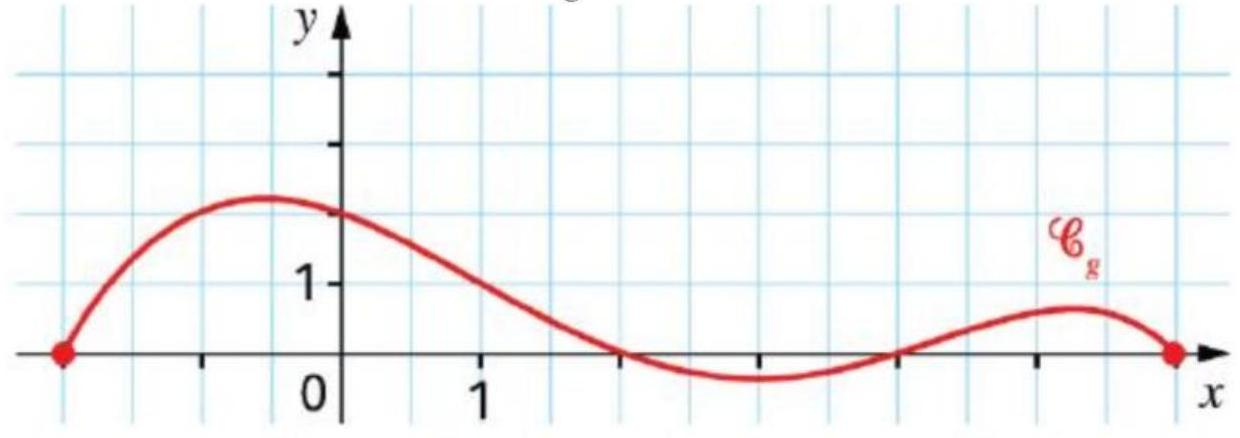
\includegraphics[scale=0.2]{2025_11_06_3b44234b8b55fbc3078dg-1(1)}
	
	\begin{enumMet}
		\item Étudier la convexité de $f$ sur $[-6 ; 6]$.
		\item Déterminer les éventuels points d'inflexion de $C_{f}$.
	\end{enumMet}
	
	\exerciceDS{ $-$ (5 points)}
	Soit $f$ la fonction définie sur $\mathbb{R}$ par:
	
	$$
	f(x)=3x^{4}-2 x^{3}-4 x^{2}
	$$
	
%	\begin{multicols}{2}
		\begin{enumMet}
			\item Calculer $f^{\prime \prime}(x)$ et étudier son signe.
			\item Étudier la convexité de $f$ sur $\mathbb{R}$.
			\item Donner les coordonnées du ou des points d'inflexion
		\end{enumMet}
%	\end{multicols}
	
	\exerciceDS{ $-$ (5 points)}
	Soit $f$ la fonction définie sur \R par:
	
	$$
	f(x)=\frac{5}{2x+6}
	$$
	
%	\begin{multicols}{2}
		\begin{enumMet}
			\item Déterminer la valeur interdite de la fonction f
			\item Étudier les variations de $f'$. 
			\item En déduire la convexité de $f$.
		\end{enumMet}
%	\end{multicols}
	
	\newpage
	\exerciceDS{ \ding{46} $-$ (5 points)}
	Soient les fonctions $f$ et $g$ définies sur $\mathbb{R}$ par:
	
	$$
	\begin{gathered}
		f(x)=3 x^{2}-5 x-3 \\
		\text { et } g(x)=-2x^{2}+2x+4
	\end{gathered}
	$$
	
	\begin{enumMet}
		\item \ding{46} On a obtenu à la calculatrice les courbes représentatives de $f$ et $g$ ci-contre. Après les avoir repérées, conjecturer si $f$, puis $g$, est convexe ou concave sur $\mathbb{R}$.
		\begin{center}
			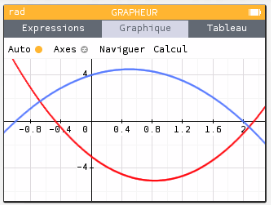
\includegraphics[scale=0.85]{Img-DS-01}
		\end{center}
		
		\item \begin{enumMet}
			\item \ding{46} Calculer $f^{\prime}(x)$, puis $f^{\prime \prime}(x)$.
			\item \ding{46} Calculer $g^{\prime}(x)$, puis $g^{\prime \prime}(x)$.
		\end{enumMet}
		\item \ding{46} Démontrer les conjectures émises.
	\end{enumMet}
	
	\exerciceDS{ $-$ (3 points)}
	On considère une fonction $f$ définie sur $\mathbb{R}$.\\
	Dans chacun des cas suivants, déterminer si la fonction $f$ est convexe ou concave sur $\mathbb{R}$.
	
	\begin{multicols}{2}
		\begin{enumMet}
			\item $f(x)=-2x^{4}-3 x^2+5x$
			\item $f(x)=2 \mathrm{e}^{-3 x}+4x^2$
		\end{enumMet}
	\end{multicols}
	
\end{document}

